% !TeX program = lualatex
% !TeX recipe = lualatex + bibtex
% CU Boulder Physics Department — Gemini Poster Template
% 35.61" x 47.48" landscape poster using Gemini beamer theme
%
% This template uses fontspec and requires LuaLaTeX or XeLaTeX:
%   lualatex poster && bibtex poster && lualatex poster && lualatex poster

\documentclass[final]{beamer}
\usepackage[orientation=landscape, size=custom, width=120.60, height=90.45, scale=1.0]{beamerposter}
% Width=47.48in=120.60cm, Height=35.61in=90.45cm (fits 36" roll printers without scaling)

\usetheme{gemini}
\usecolortheme{cuboulder}

\usepackage{amsmath, amssymb}
\usepackage{graphicx}
\usepackage{booktabs}
\hypersetup{hidelinks}
\usepackage[backend=bibtex, style=numeric-comp, maxnames=3]{biblatex}
\addbibresource{references.bib}

% ============================================================
% === CONFIGURATION — EDIT THIS SECTION ===
% ============================================================

% Poster metadata
\title{Your Poster Title Goes Here}
\author{Author One \inst{1} \samelineand Author Two \inst{2} \samelineand Author Three \inst{1}}
\institute[shortinst]{
  \inst{1} Department of Physics, University of Colorado Boulder \samelineand
  \inst{2} JILA, University of Colorado Boulder
}

% Logo paths (relative to this file)
% To use only one logo, comment out the other with %
\logoleft{\includegraphics[height=3.5cm]{../assets/Boulder_left_lockup_rev_2025.png}}
\logoright{\includegraphics[height=3.5cm]{../assets/Physics_rev_left.png}}

% Footer content (comment out to remove the footer entirely)
\footercontent{
  \href{mailto:author@colorado.edu}{author@colorado.edu} \hfill
  ABC Conference 2026, City \hfill
  \href{https://www.colorado.edu}{https://www.colorado.edu}
}

% Column layout
\newlength{\sepwidth}
\newlength{\colwidth}
\setlength{\sepwidth}{0.025\textwidth}
\setlength{\colwidth}{0.3\textwidth}

\newcommand{\separatorcolumn}{\begin{column}{\sepwidth}\end{column}}

% ============================================================
% === DOCUMENT ===
% ============================================================

\begin{document}
\begin{frame}[t]

\begin{columns}[T]

\separatorcolumn

% === COLUMN 1 ===
\begin{column}{\colwidth}

\begin{block}{Introduction}
  Lorem ipsum dolor sit amet, consectetur adipiscing elit. Morbi accumsan
  fermentum magna, vel pretium arcu fermentum ac. Nunc pellentesque eros sed
  ligula ultrices varius. Integer vel nunc et mi porta
  eleifend~\cite{einstein1905}.

  \begin{itemize}
    \item Lorem ipsum dolor sit amet, consectetur adipiscing elit
    \item Pellentesque ultricies velit in fermentum vestibulum
    \item Nunc a lectus et eros facilisis hendrerit eu non urna
  \end{itemize}
\end{block}

\begin{block}{Theoretical Framework}
  The spectral energy density $u(\nu, T)$ is given by:
  \begin{equation}
    u(\nu, T) = \frac{8\pi h\nu^3}{c^3} \frac{1}{e^{h\nu/k_B T} - 1}
    \label{eq:planck}
  \end{equation}
  where $h$ is Planck's constant, $\nu$ is frequency, $c$ is the speed of
  light, and $k_B$ is Boltzmann's constant. In the low-frequency limit
  ($h\nu \ll k_B T$), this reduces to the Rayleigh--Jeans approximation
  $u(\nu, T) \approx 8\pi\nu^2 k_B T / c^3$.

  \begin{itemize}
    \item In the high-frequency regime, the exponential cutoff dominates
    \item At low frequencies, the classical approximation holds
    \item The peak frequency $\nu_{\max}$ shifts linearly with temperature
  \end{itemize}
\end{block}

\begin{block}{Methods}
  Lorem ipsum dolor sit amet, consectetur adipiscing elit. Curabitur
  condimentum sem id semper vulputate. Nam lobortis ultrices iaculis.
  Maecenas bibendum, sem vel vehicula tempus, nisi tortor eleifend tellus.

  \begin{itemize}
    \item Duis finibus finibus sapien, ut mollis odio malesuada
    \item Aenean ut ex augue, quisque vulputate scelerisque eros
    \item Proin ultrices sodales nulla eu molestie nullam
  \end{itemize}

  Lorem ipsum dolor sit amet, consectetur adipiscing elit. Morbi accumsan
  fermentum magna, vel pretium arcu fermentum ac~\cite{higgs2012}. Nunc
  pellentesque eros sed ligula ultrices varius. Integer vel nunc et mi porta
  eleifend. Praesent eget felis a ante facilisis viverra non ut lacus.
\end{block}

\end{column}

\separatorcolumn

% === COLUMN 2 ===
\begin{column}{\colwidth}

\begin{block}{Experimental Setup}
  \begin{figure}
    \centering
    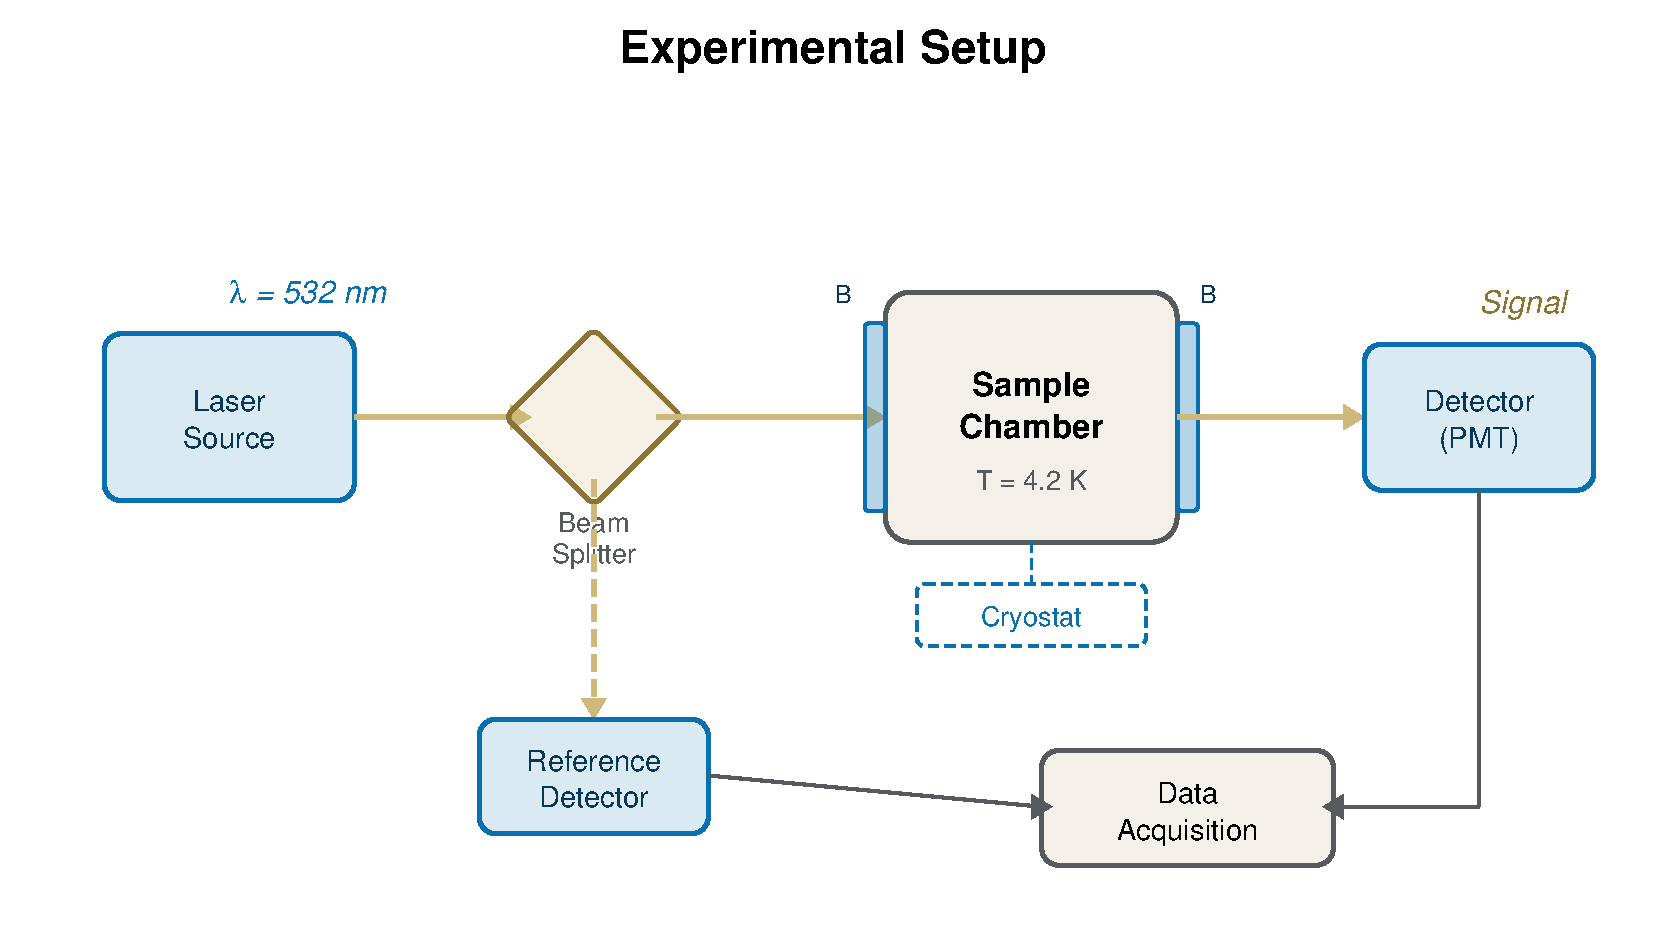
\includegraphics[width=0.9\columnwidth]{../assets/example-diagram.pdf}
    \caption{Schematic of the experimental apparatus.}
    \label{fig:setup}
  \end{figure}
\end{block}

\begin{alertblock}{Results}
  Lorem ipsum dolor sit amet, consectetur adipiscing elit. Sed non risus.
  Suspendisse lectus tortor, dignissim sit amet, adipiscing nec, ultricies
  sed dolor. See Fig.~\ref{fig:setup} and Table~\ref{tab:results}.

  \begin{table}
    \centering
    \caption{Summary of measured experimental parameters.}
    \label{tab:results}
    \begin{tabular}{lcc}
      \toprule
      \textbf{Parameter} & \textbf{Value} & \textbf{Uncertainty} \\
      \midrule
      Sample temperature (K) & 4.21 & $\pm\,0.05$ \\
      Applied field (T) & 1.50 & $\pm\,0.01$ \\
      Resonance frequency (GHz) & 9.38 & $\pm\,0.02$ \\
      Linewidth (MHz) & 12.7 & $\pm\,0.3$ \\
      Signal-to-noise ratio & 42.0 & $\pm\,1.5$ \\
      \bottomrule
    \end{tabular}
  \end{table}

  The measured spectral distribution is consistent with the theoretical
  prediction from Eq.~\eqref{eq:planck}, confirming the validity of the
  model across the full frequency range examined.
\end{alertblock}

\begin{block}{Data Analysis}
  Pellentesque habitant morbi tristique senectus et netus et malesuada fames
  ac turpis egestas. Fusce aliquet pede non pede. Suspendisse dapibus lorem
  pellentesque magna~\cite{arxiv_example}.

  Lorem ipsum dolor sit amet, consectetur adipiscing elit. Morbi accumsan
  fermentum magna, vel pretium arcu fermentum ac. Nunc pellentesque eros sed
  ligula ultrices varius. Integer vel nunc et mi porta eleifend.
\end{block}

\end{column}

\separatorcolumn

% === COLUMN 3 ===
% To switch to a 2-column layout:
%   1. Change \colwidth to 0.45\textwidth
%   2. Move Column 3 content into Column 1 or 2
%   3. Delete the Column 3 section below
\begin{column}{\colwidth}

\begin{block}{Data Analysis (continued)}
  \begin{figure}
    \centering
    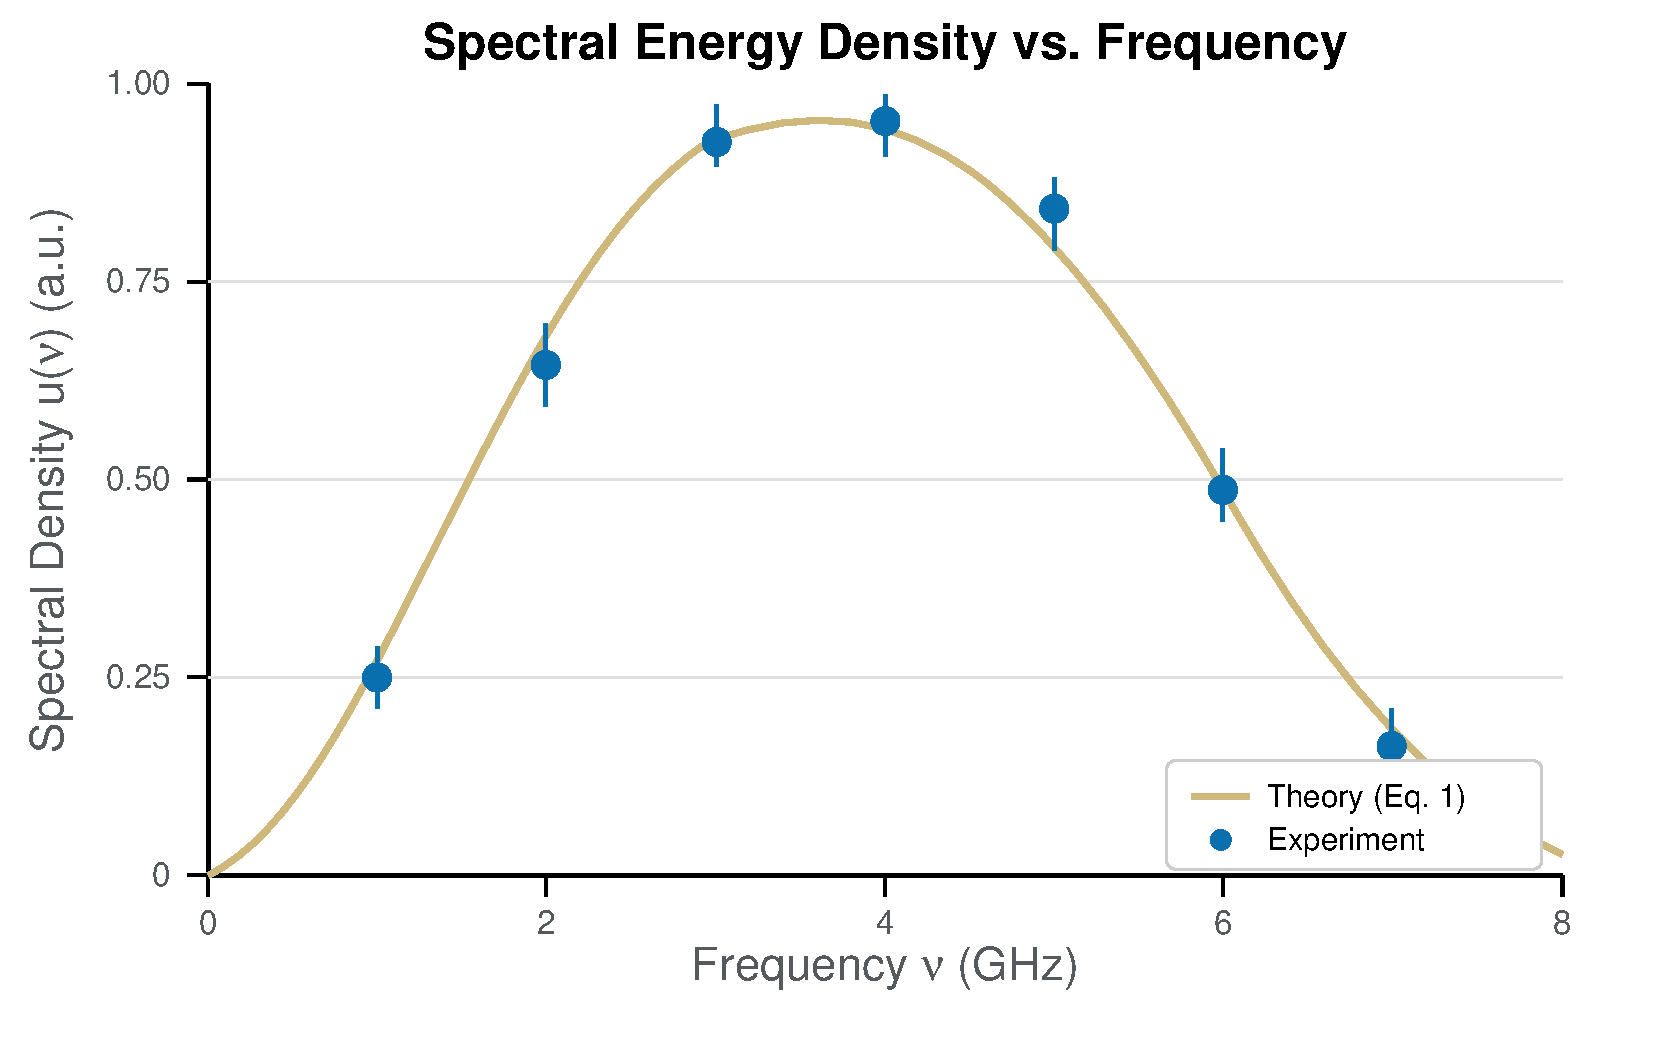
\includegraphics[width=0.9\columnwidth]{../assets/example-plot.pdf}
    \caption{Measured values as a function of the control parameter. The gold
    line shows the theoretical prediction from Eq.~\eqref{eq:planck}; blue
    points are experimental data with error bars.}
    \label{fig:result}
  \end{figure}
\end{block}

\begin{alertblock}{Central Result}
  Lorem ipsum dolor sit amet, consectetur adipiscing elit. Vivamus congue
  volutpat elit non semper. Phasellus mauris felis, molestie ac pharetra
  quis, tempus nec ante.
\end{alertblock}

\begin{block}{Discussion}
  Lorem ipsum dolor sit amet, consectetur adipiscing elit. Cras imperdiet vel
  elit dignissim cursus. As shown in Eq.~\eqref{eq:planck} and
  Fig.~\ref{fig:result}, the results are consistent with our initial
  hypothesis~\cite{griffiths2018}.

  \begin{itemize}
    \item Sed luctus elit sit amet dictum maximus
    \item Pellentesque facilisis dolor in leo bibendum congue
    \item Maecenas congue finibus justo, vitae eleifend urna facilisis at
  \end{itemize}
\end{block}

\begin{exampleblock}{Main Conclusion}
  Lorem ipsum dolor sit amet, consectetur adipiscing elit. Donec finibus ante
  vel purus mollis fermentum~\cite{conference_example}.
\end{exampleblock}

\begin{block}{References}
  \nocite{*}
  \printbibliography[heading=none]
\end{block}

\begin{block}{Acknowledgments}
  This work was supported by the National Science Foundation (Grant
  No.~PHY-XXXXXXX). We thank Prof.~A.~B.~Smith for valuable discussions,
  the CU Boulder Department of Physics machine shop for technical support,
  and Dr.~C.~D.~Jones for assistance with data analysis. Additional thanks
  to the CU Boulder Department of Physics for poster printing resources.
\end{block}

\end{column}

\separatorcolumn

\end{columns}

\end{frame}
\end{document}
